\documentclass[10pt]{beamer}

\title{A5 Group CAD \\Project Gemini}
\author{Ahmed Woodson, Mark DeVince, Charles Hanner, Blaire Weinberg, Hyunsoo Chun}
\date{\today}

\graphicspath{{./Images/}}


\begin{document}
	\frame{\titlepage}
	
	\section{Group}
	
	\begin{frame}{Group Beauty Shot}
\begin{minipage}{0.49\textwidth}
	\begin{itemize}
		\item Gemini was a 2 crew Apollo proving ground
		\item Launch mass was 3.8 MT, with 455 kg of propellant
		\item 12 Gemini flights were flown, with duration between 5 hours and 14 days
	\end{itemize}
\end{minipage}%
\begin{minipage}{0.49\textwidth}
	\begin{figure}
		\centering
		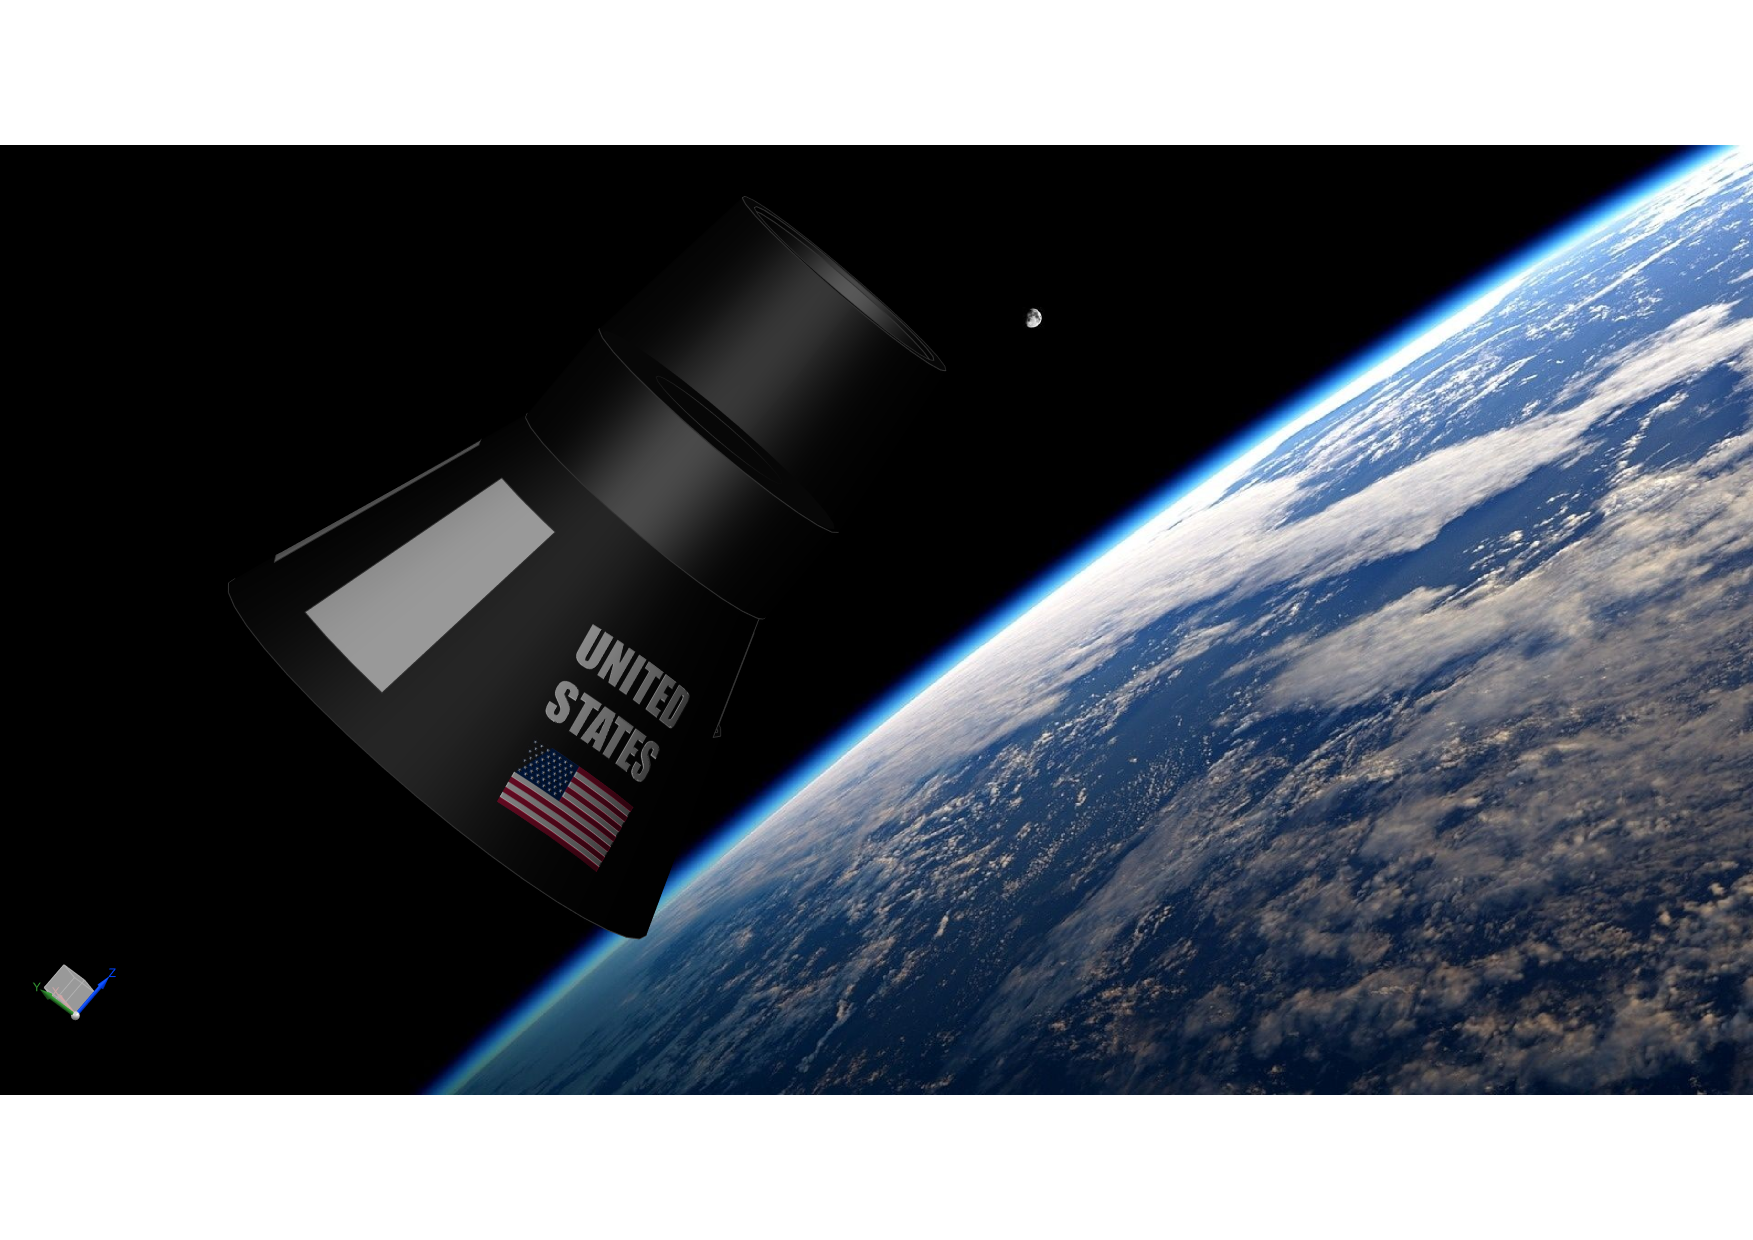
\includegraphics[width=\textwidth]{Group_Beauty.png}
	\end{figure}
	
\end{minipage}
\end{frame}

\begin{frame}{External 3 View}
\begin{figure}
	\centering
	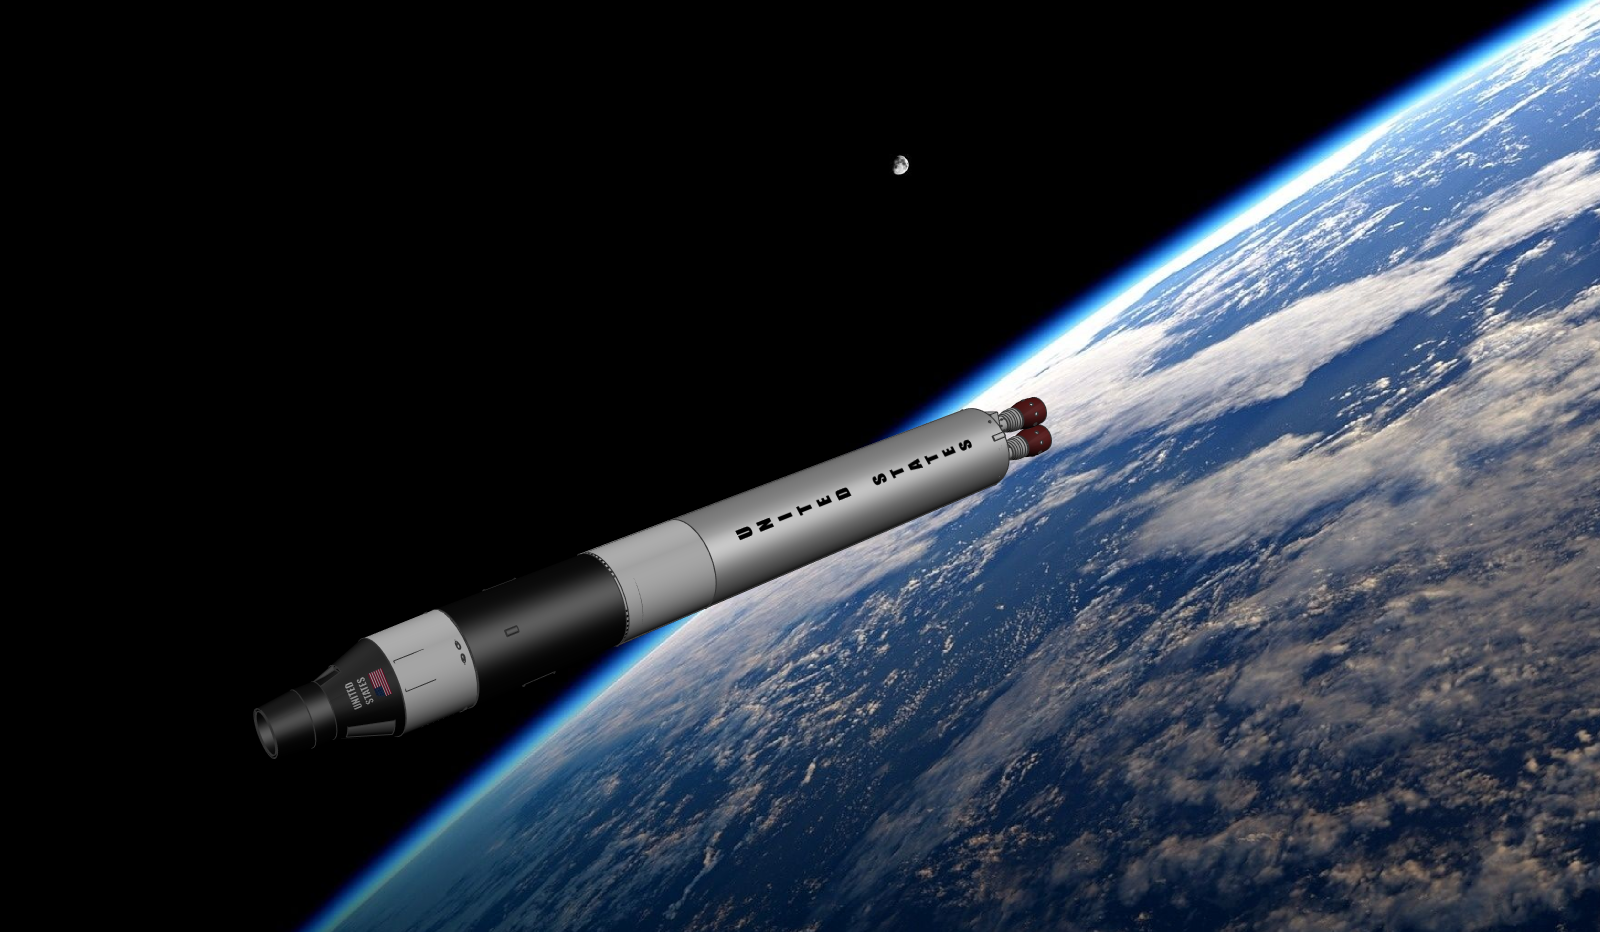
\includegraphics[width=0.5\textwidth]{External_3_View.png}
\end{figure}
\end{frame}

	\begin{frame}{Interior View}
\begin{figure}
	\centering
	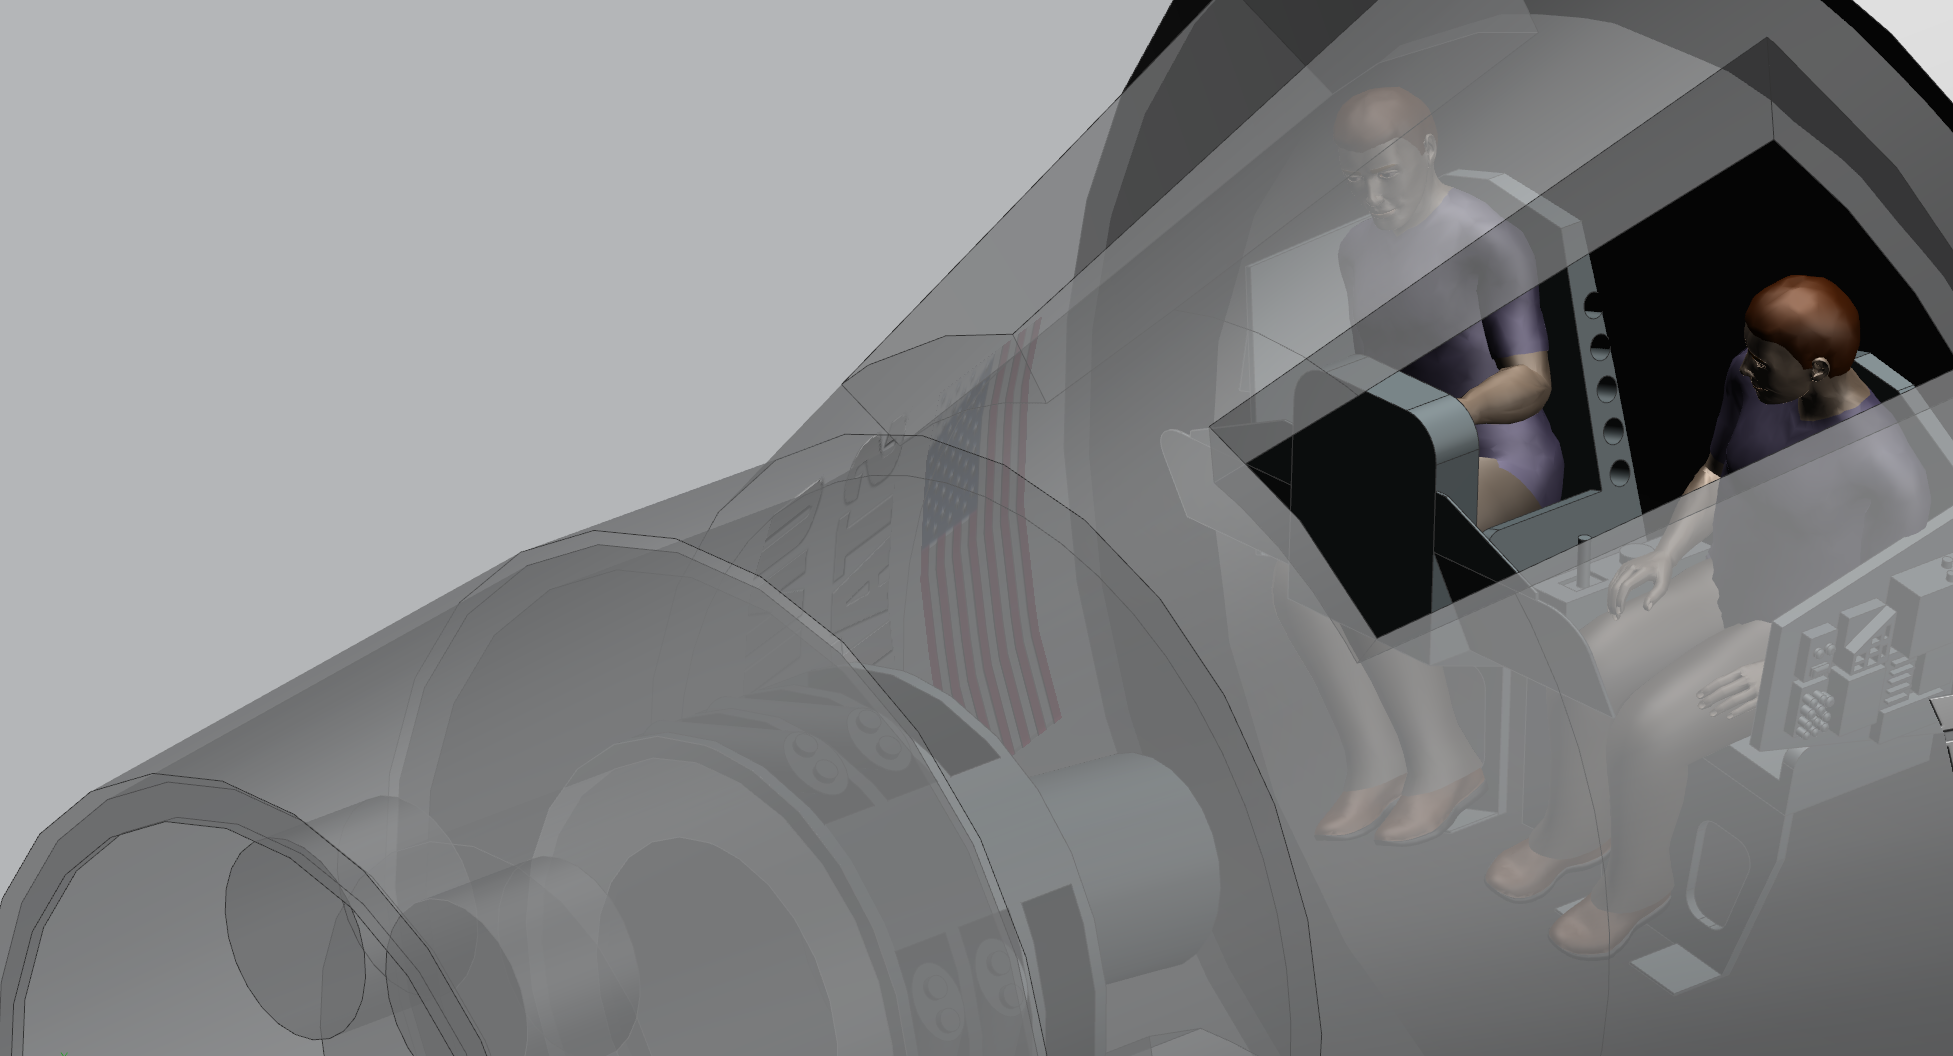
\includegraphics[width=0.5\textwidth]{Interior_View.png}
\end{figure}
\end{frame}

	\begin{frame}{Color Coded}
\begin{minipage}{0.4\textwidth}
\begin{table}
	\begin{tabular}{|c|c|}\hline
		\textbf{Person} & \textbf{Color}\\ \hline
		Ahmed Woodson & Blue\\ \hline
		Mark DeVince & {}\\  \hline
		Charles Hanner & Green\\ \hline
		Blaire Weinberg & Grey\\  \hline
		Hyunsoo Chun & Red\\ \hline
	\end{tabular}
\end{table}	
\end{minipage}%
\begin{minipage}{0.59\textwidth}
	\begin{figure}
		\centering
		
\includegraphics[width=\textwidth]{Color_Coded.png}
	\end{figure}
\end{minipage}
\end{frame}
	\begin{frame}{Launch Vehicle}
\begin{figure}
	\centering
	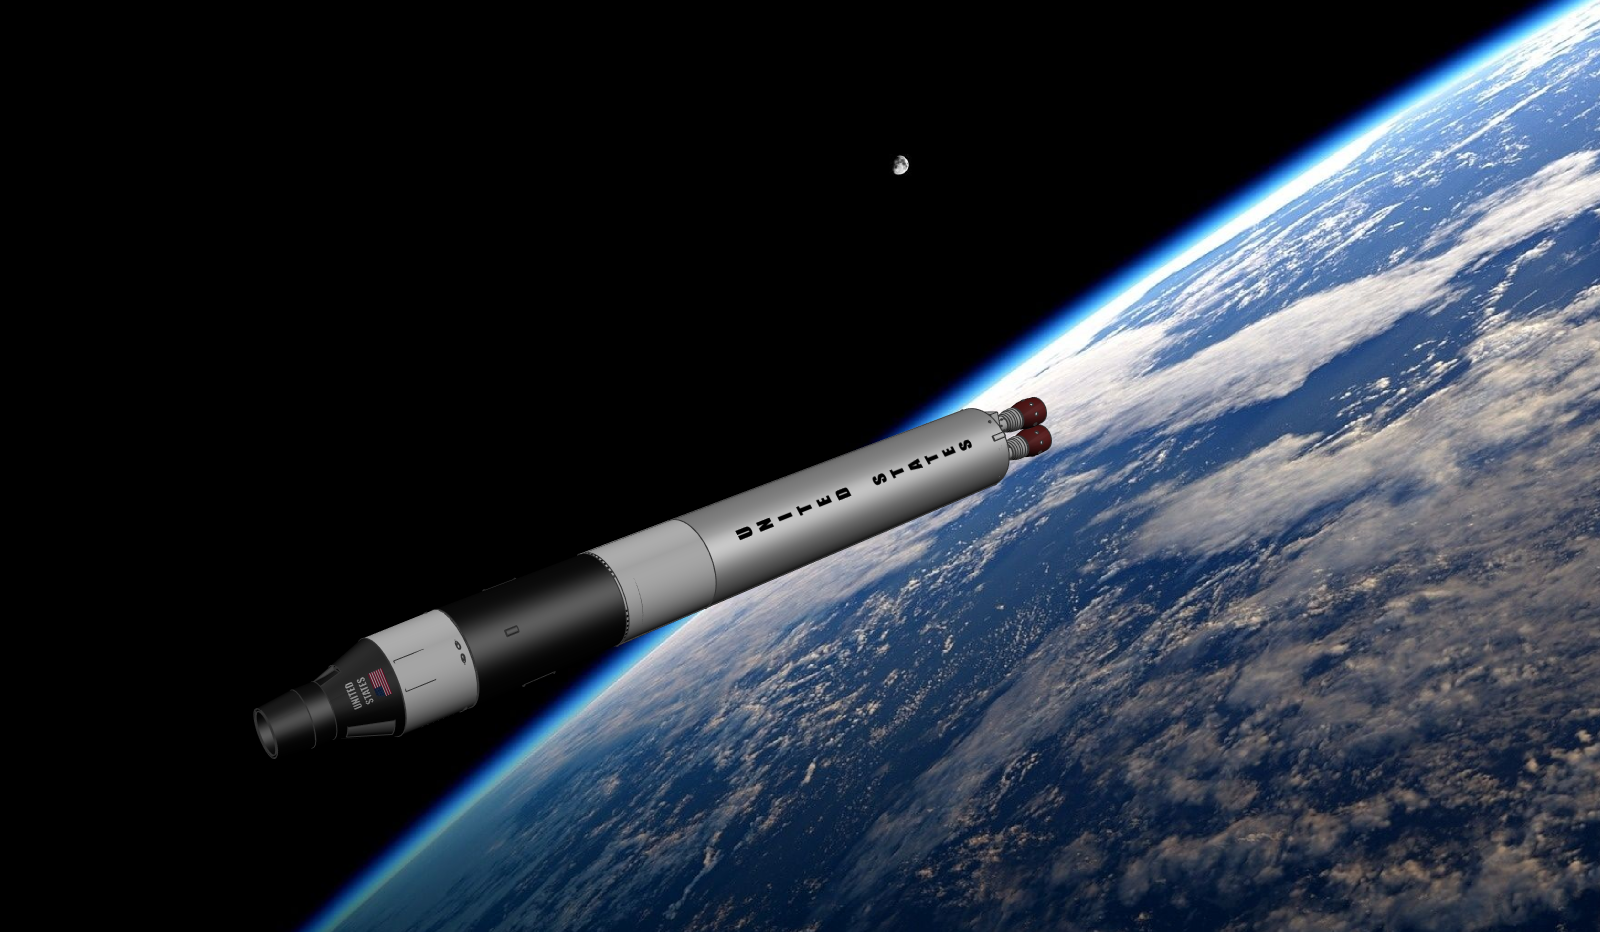
\includegraphics[width=0.5\textwidth]{Launch_Vehicle.png}
\end{figure}
\end{frame}

	\begin{frame}{Baseball Card}
	\begin{minipage}{0.49\textwidth}
\begin{itemize}
	\item A total of 12 Gemini spacecraft flew, the first two being uncrewed
	\item The Gemini Program was mean to be a proving ground for Apollo, and included testing things like spacewalks and rendezvous and docking
	\item Gemini launched on a modified Titan II ICBM from Pad-19 in Cape Canaveral, FL
\end{itemize}
	\end{minipage}%
\begin{minipage}{0.49\textwidth}
	\begin{figure}
		\centering
		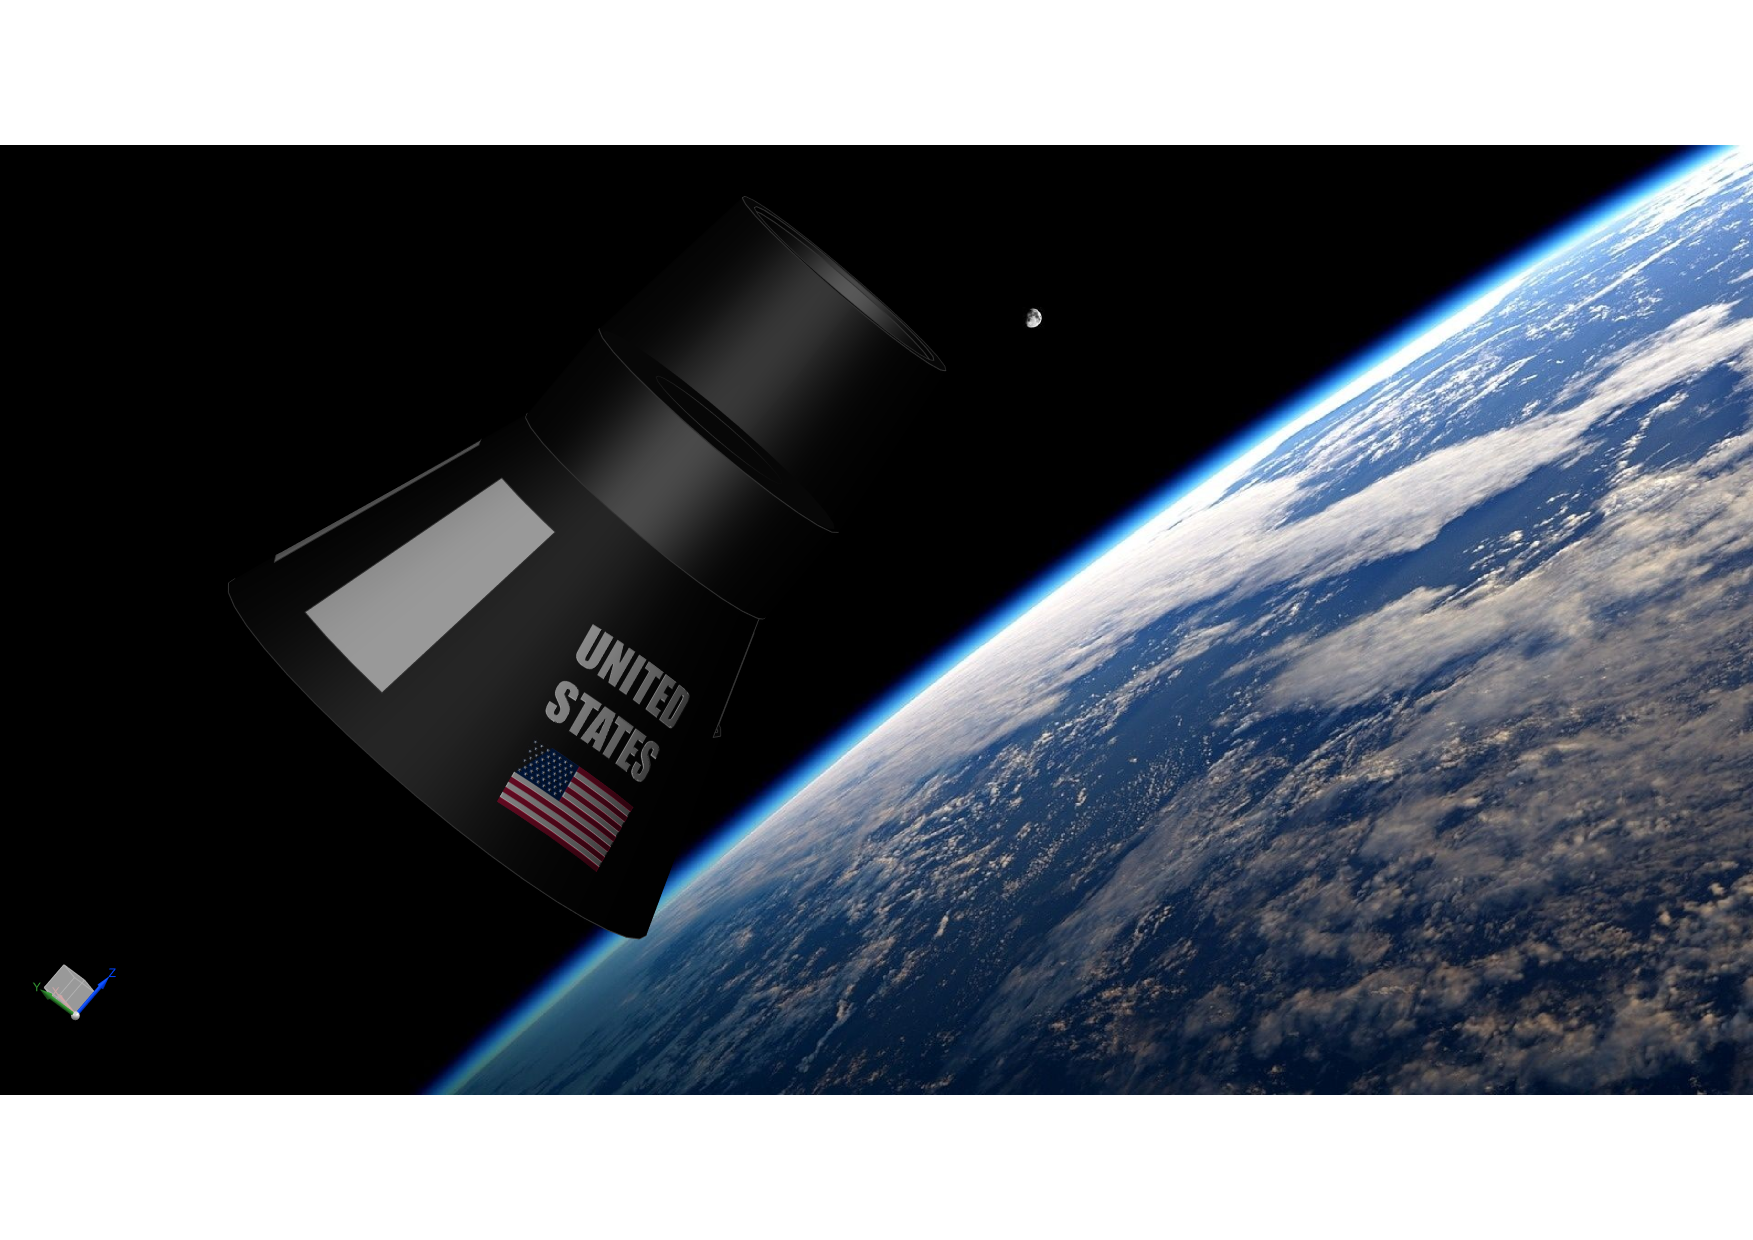
\includegraphics[width=\textwidth]{Group_Beauty.png}
	\end{figure}
	
\end{minipage}

\end{frame}

\section{individual}


	\begin{frame}{Woodson: Beauty Shot}
\begin{figure}
	\centering
	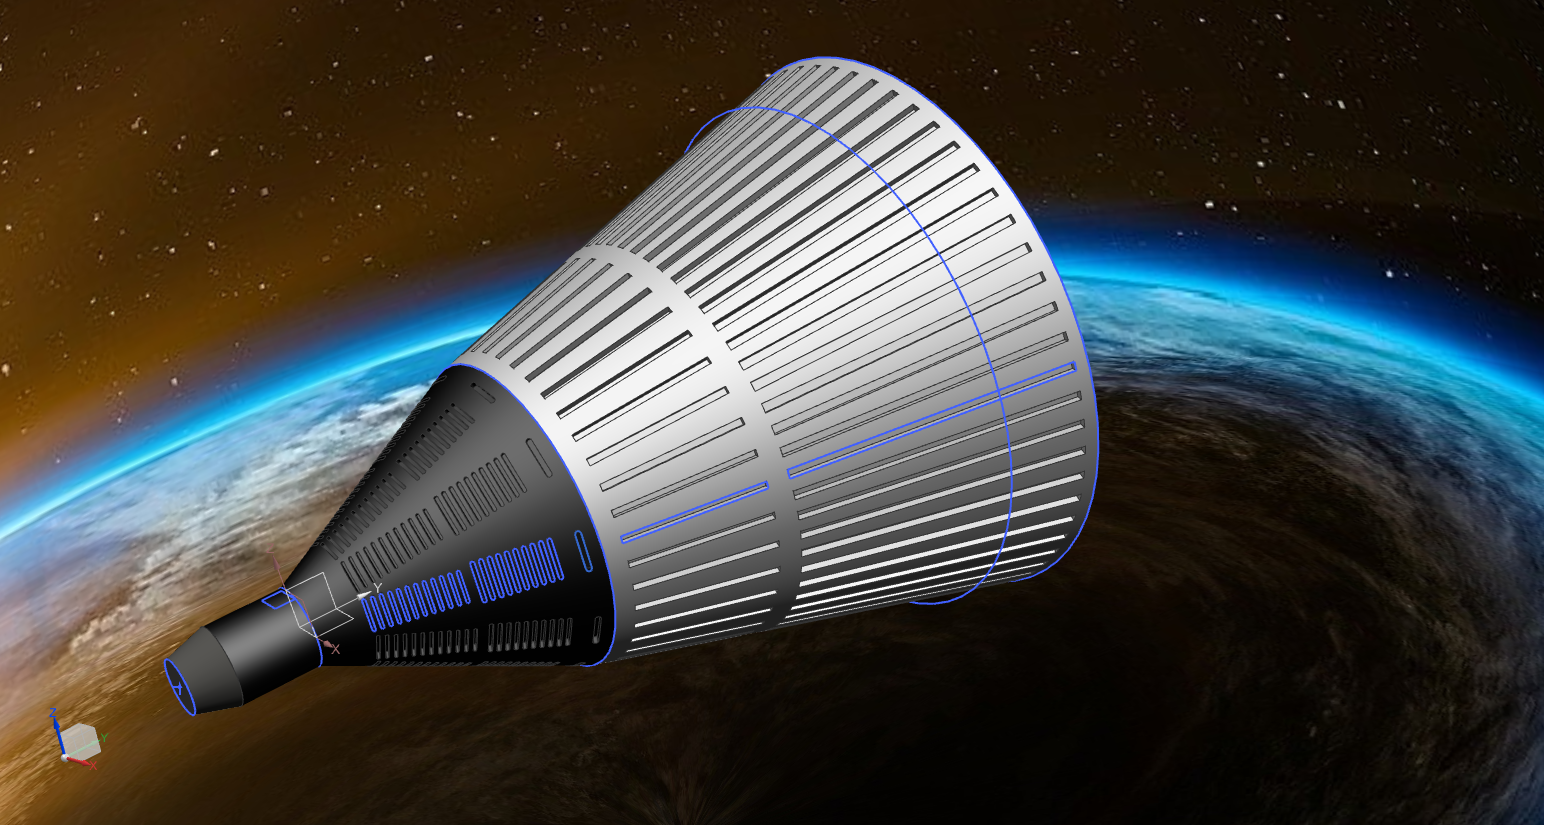
\includegraphics[width=0.5\textwidth]{Woodson_Beauty.png}
\end{figure}
\end{frame}

	\begin{frame}{Woodson: 3 View}
\begin{figure}
	\centering
	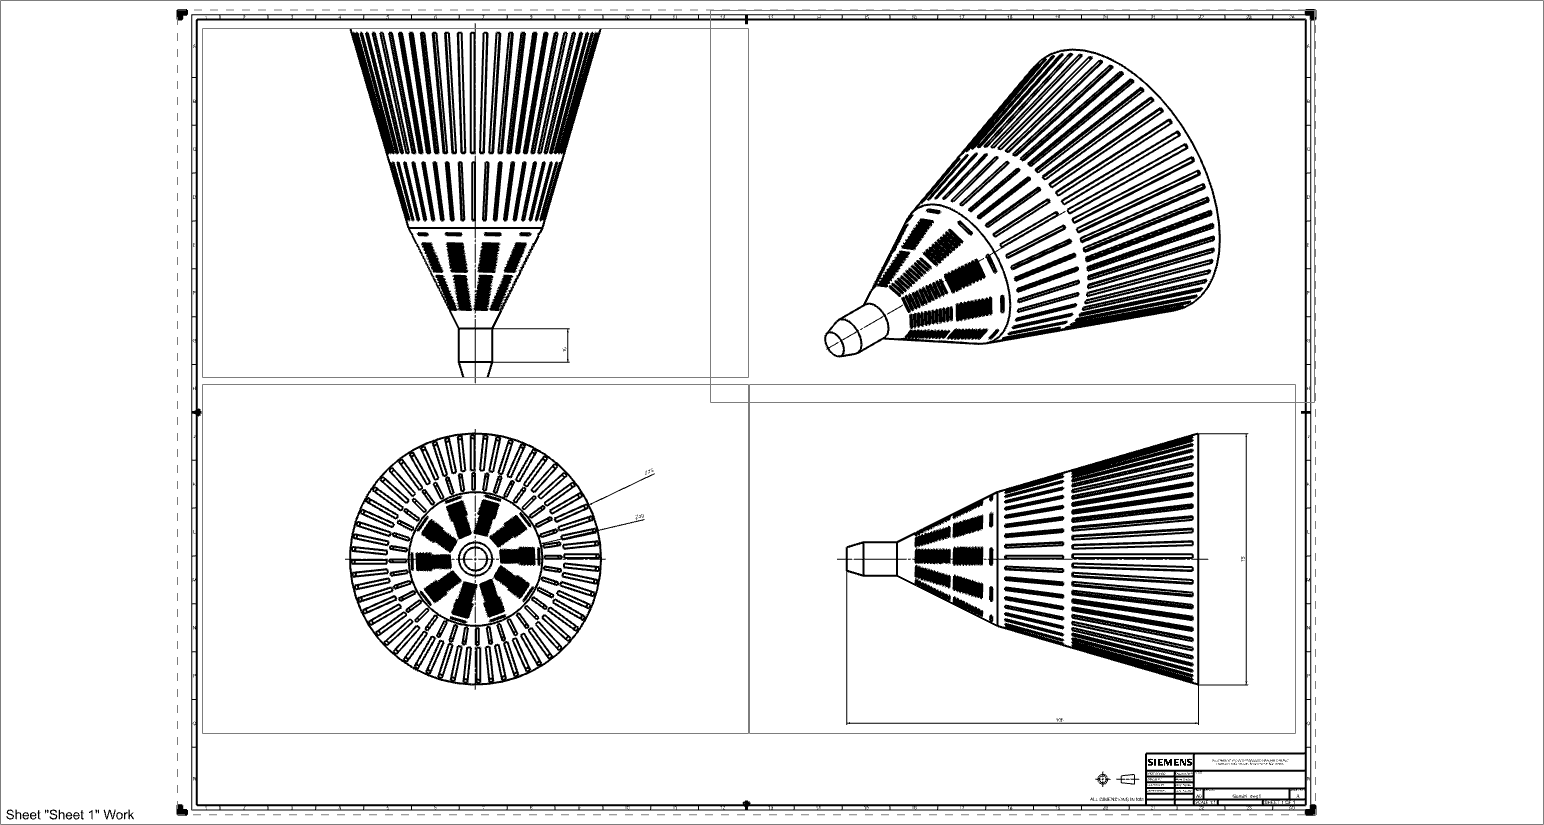
\includegraphics[width=0.5\textwidth]{Woodson_3_View.png}
\end{figure}
\end{frame}

	\begin{frame}{DeVince: Beauty Shot}
\begin{figure}
	\centering
	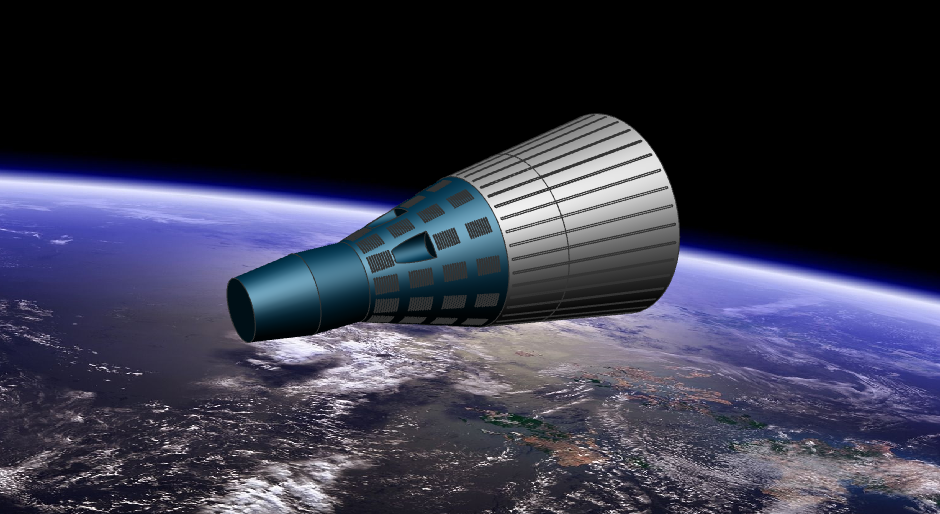
\includegraphics[width=0.5\textwidth]{DeVince_Beauty.png}
\end{figure}
\end{frame}

\begin{frame}{DeVince: 3 View}
\begin{figure}
\centering
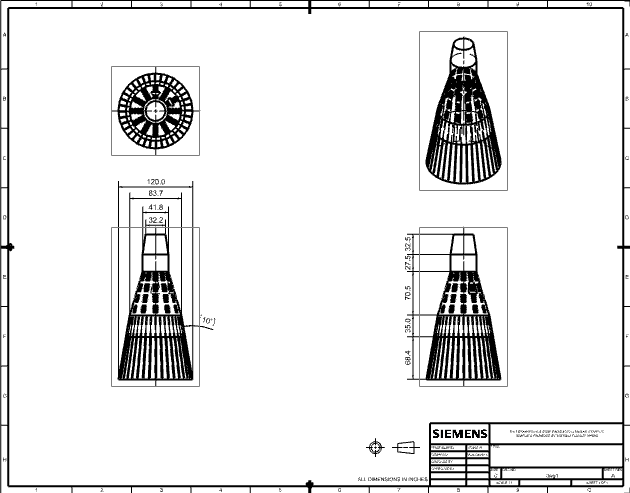
\includegraphics[width=0.5\textwidth]{DeVince_3_View.png}
\end{figure}
\end{frame}

	\begin{frame}{Hanner: Beauty Shot}
\begin{figure}
	\centering
	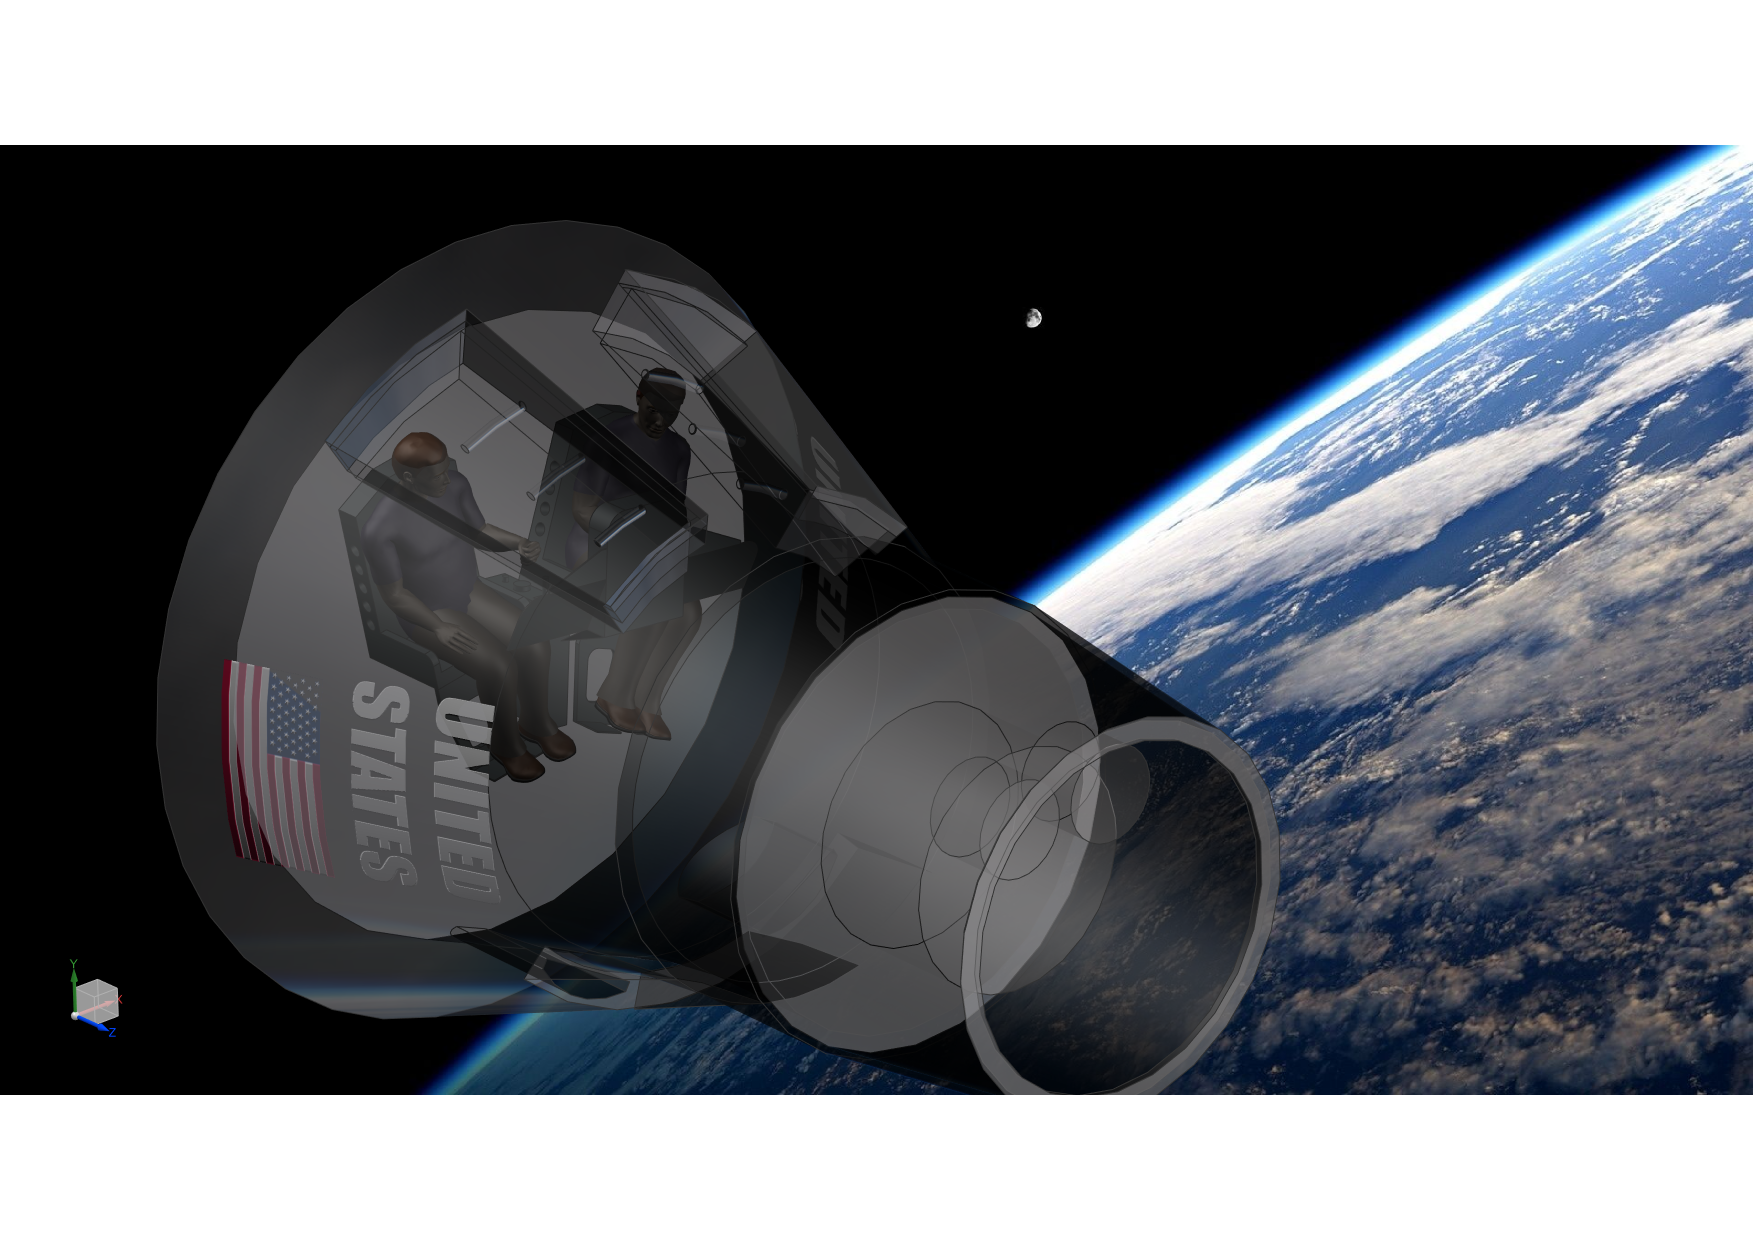
\includegraphics[width=0.5\textwidth]{Hanner_Beauty.png}
\end{figure}
\end{frame}

\begin{frame}{Hanner: 3 View}
\begin{figure}
\centering
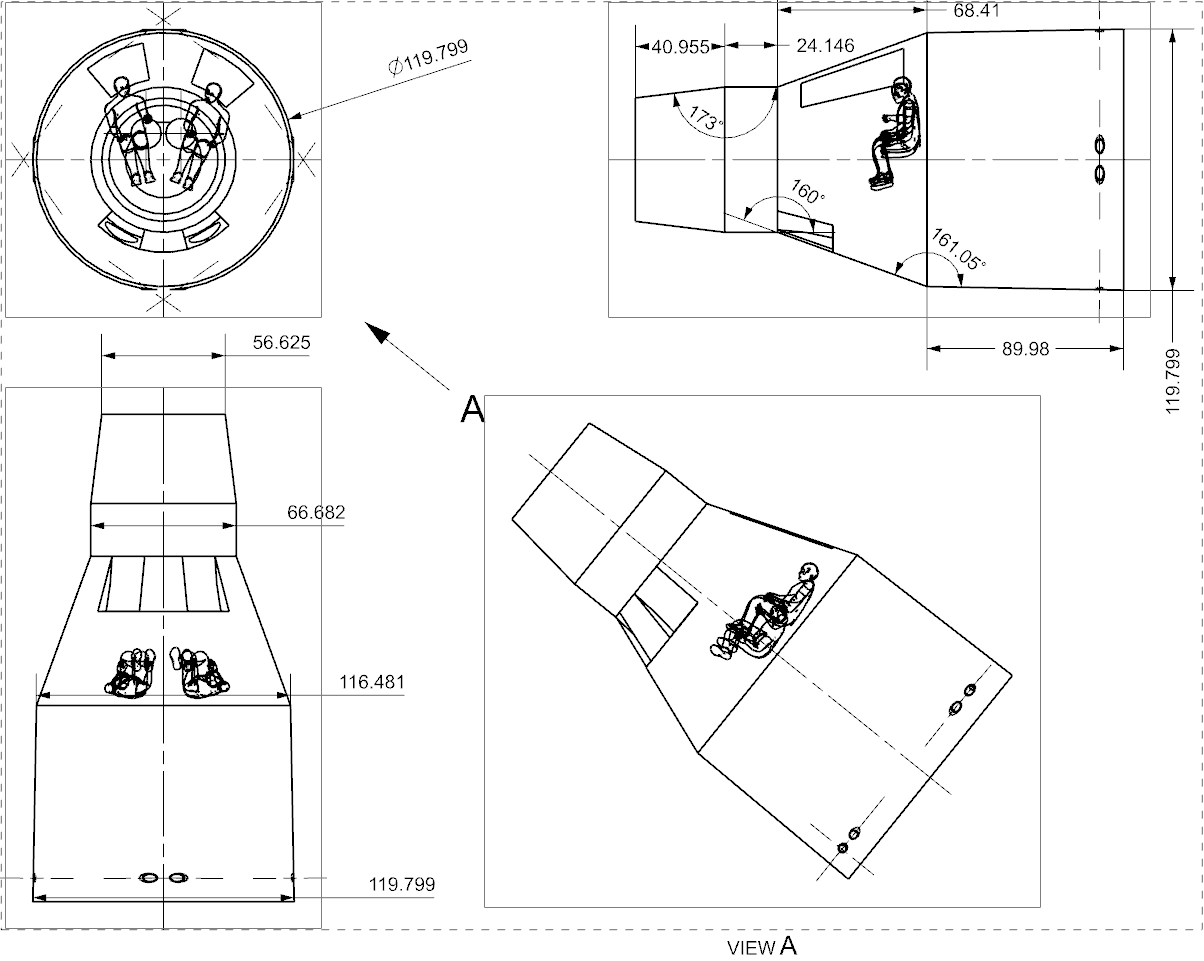
\includegraphics[width=0.5\textwidth]{Hanner_3_View.png}
\end{figure}
\end{frame}

	\begin{frame}{Weinberg: Beauty Shot}
\begin{figure}
	\centering
	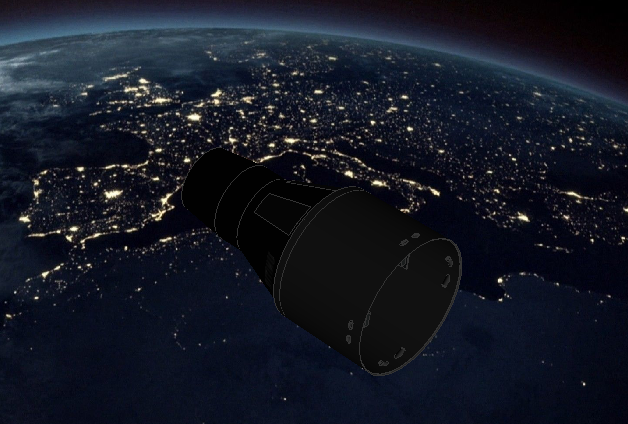
\includegraphics[width=0.5\textwidth]{Weinberg_Beauty.png}
\end{figure}
\end{frame}

\begin{frame}{Weinberg: 3 View}
\begin{figure}
\centering
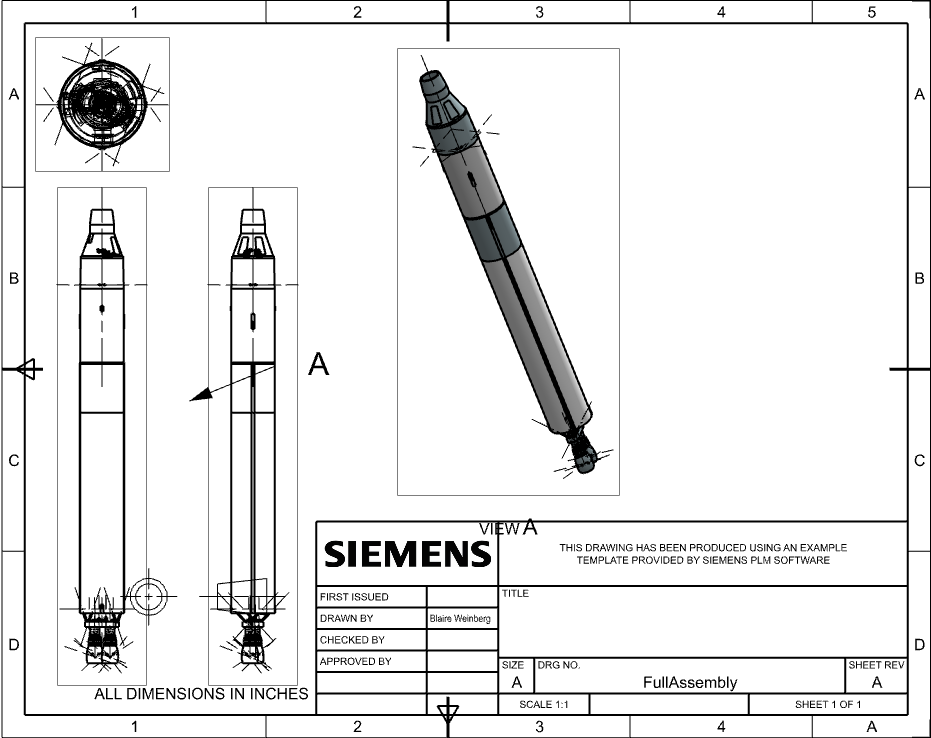
\includegraphics[width=0.5\textwidth]{Weinberg_3_View.png}
\end{figure}
\end{frame}

	\begin{frame}{Chun: Beauty Shot}
\begin{figure}
	\centering
	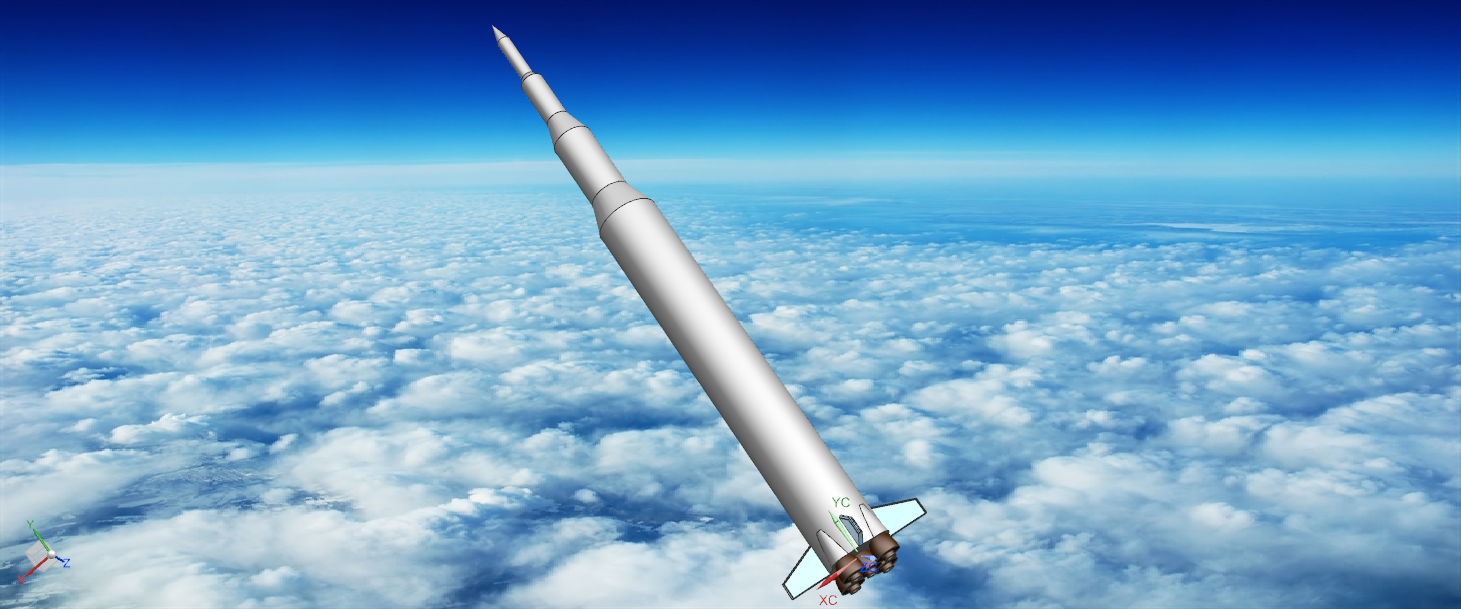
\includegraphics[width=0.5\textwidth]{Chun_Beauty.png}
\end{figure}
\end{frame}

\begin{frame}{Chun: 3 View}
\begin{figure}
\centering
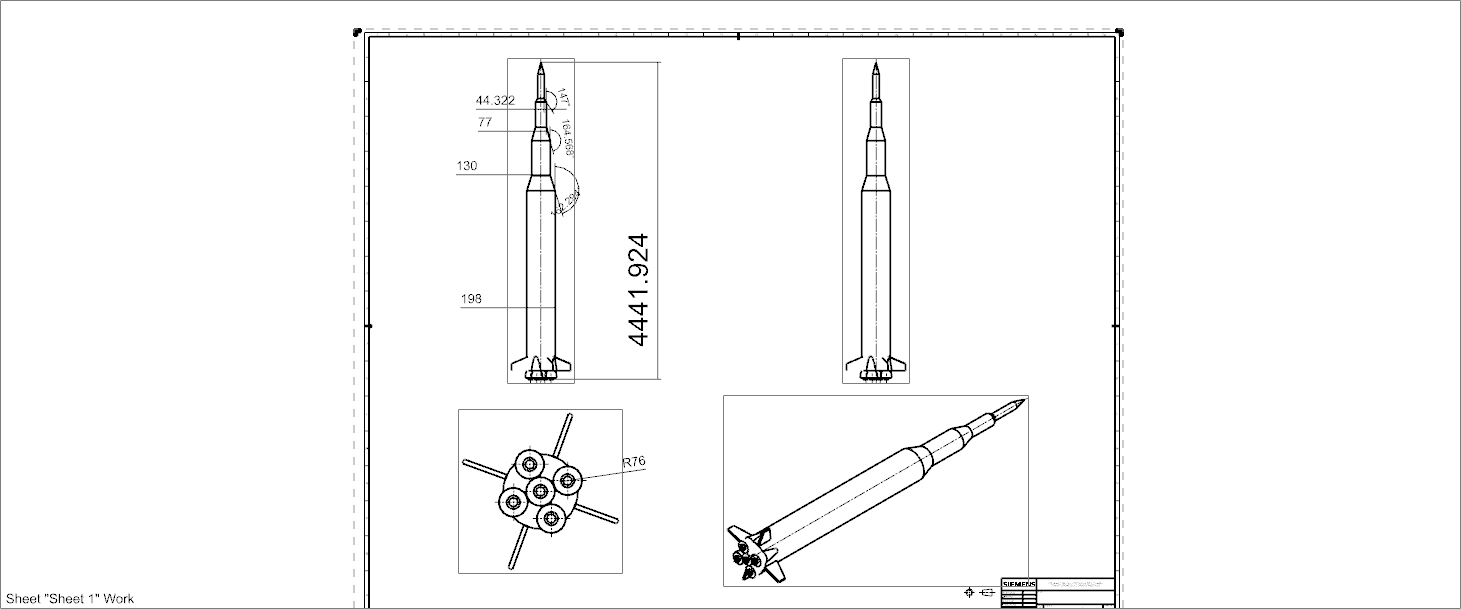
\includegraphics[width=0.5\textwidth]{Chun_3_View.png}
\end{figure}
\end{frame}
\end{document}

